\documentclass[aspectratio=169,usenames,dvipsnames]{beamer}

\usepackage{pgf}  
\usepackage{tikz}
\usetikzlibrary{arrows}
\usepgflibrary{shapes.arrows} 
\usetikzlibrary{intersections}
\usetikzlibrary{calc}
\usetikzlibrary{fit}
\usetikzlibrary{automata,positioning}
\usepackage{pgfplots,stackengine}
\usepackage{fontspec}
\usepackage{fancyvrb}
\usepackage{wasysym}
\usepackage{unicode-math}
\usepackage{import}
\usepackage{rotating}
\usepackage{gensymb}
\usepackage{chemfig}
\usepackage{rotating}
\usepackage{booktabs}
\usepackage{pifont}
\usepackage{wrapfig}
\usepackage{mathtools}
\usepackage{graphbox}
\usepackage{epigraph}
\usepackage{listings}
\usepackage{verbatim}
\usepackage{hologo}
\usepackage{wrapfig}
\usepackage[absolute,overlay]{textpos}
\usepackage[euler-digits,euler-hat-accent]{eulervm}
%\logo{\pgfputat{\pgfxy(.45,.5)}{\pgfbox[center]{
\includegraphics[width=1.7cm]{Figures/uu_shadow.pngu}}}}

\usetheme{Copenhagen}
\usecolortheme{beaver}

\definecolor{uured}{RGB}{153,0,0}
\setbeamercolor{block title}{use=structure,fg=white,bg=uured}
\setbeamercolor*{item}{fg=red}

\newcommand{\unilogo}{
  \setlength{\TPHorizModule}{1pt}
  \setlength{\TPVertModule}{1pt}
  \begin{textblock}{1}(26,-10)
   
\includegraphics[height=70pt, align=c]{Figures/uu_shadow.png}
  \end{textblock}
  } 

\pgfmathdeclarefunction{gauss}{2}{%
  \pgfmathparse{1/(#2*sqrt(2*pi))*exp(-((x-#1)^2)/(2*#2^2))}%
}
  
\makeatletter
    \newcases{mycases}{\quad}{%
        \hfil$\m@th\displaystyle{##}$}{$\m@th\displaystyle{##}$\hfil}{\lbrace}{.}
\makeatother

\addtobeamertemplate{frametitle}{}{%
    \unilogo
}
\LetLtxMacro{\oldBlock}{\block}
\LetLtxMacro{\oldEndBlock}{\endblock}
\renewcommand{\block}{\begin{center}\begin{minipage}{0.8\textwidth}\oldBlock}
\renewcommand{\endblock}{\oldEndBlock\end{minipage}\end{center}}
\definecolor{darkpastelgreen}{rgb}{0.01, 0.75, 0.24}

\setlength{\fboxsep}{0pt}

\begin{document}
\graphicspath{{Figures/}}
\setsansfont[ItalicFont = Optima Italic,
             BoldFont = Optima Bold,
             Ligatures=TeX ]
            {Optima Regular}
\setmainfont[ItalicFont = Optima Italic,
             BoldFont = Optima Bold,
             Ligatures=TeX]
            {Optima Regular}
\newfontfamily\commentfont[]{Chalkboard}
\newfontfamily\DejaSans{DejaVuSans.ttf}
\newfontfamily\herculanum[]{Herculanum}
\newfontfamily\timesfont[ItalicFont = Times New Roman Italic]{Times New Roman}
\newcommand{\lmr}{\fontfamily{lmr}\selectfont}
\newfontfamily\zA[Ligatures={Common, Rare}, Variant=1] {Zapfino}
\newfontfamily\zB[Ligatures={Common, Rare}, Variant=2] {Zapfino}
\newfontfamily\zC[Ligatures={Common, Rare}, Variant=3] {Zapfino}
\newfontfamily\zD[Ligatures={Common, Rare}, Variant=4] {Zapfino}
\newfontfamily\zE[Ligatures={Common, Rare}, Variant=5] {Zapfino}
\newfontfamily\zF[Ligatures={Common, Rare}, Variant=6] {Zapfino}
\newfontfamily\zG[Ligatures={Common, Rare}, Variant=7] {Zapfino}
\renewcommand\UrlFont{\color{blue}}
\renewcommand\thefootnote{\textcolor{uured}{\arabic{footnote}}}
\setbeamercolor{alerted text}{fg=uured}
\lstset{basicstyle=\ttfamily\scriptsize, frame=single }
\newcommand{\TikZ}{{\lmr Ti\textit{k}Z}}

\title{Big data storage and transfer}   
\author{Jonathan Alvarsson} 
%\titlegraphic{\vfill\includegraphics[width=18em]{Figures/ORN_large.png}}
\date{\today} 

\setbeamertemplate{background}{%
    \parbox[c][\paperheight]{\paperwidth}{%
        \vfill
        \hfill
        
\includegraphics[height=0.65\textheight]{Figures/sigill.png}
    }   
}
\begin{frame}[plain]
\unilogo \vspace{1cm} \titlepage
\begin{tikzpicture}[remember picture,overlay]
\tikz[remember picture, overlay] \fill[uured] (current page.north west) rectangle ++(\paperwidth,-0.5cm);
\end{tikzpicture}%
\end{frame}

\setbeamertemplate{background}{}
\renewcommand{\unilogo}{
  \setlength{\TPHorizModule}{1pt}
  \setlength{\TPVertModule}{1pt}
  \begin{textblock}{1}(0,0)
   
\includegraphics[height=27pt, align=c]{Figures/uu.png}
  \end{textblock}
  } 

{
    \setbeamercolor{background canvas}{bg=black}
    \setbeamercolor{normal text}{fg=white}\usebeamercolor*{normal text}
    \setbeamercolor{item}{fg=white, bg=black}

    \begin{frame}[plain]
        \begin{center}
        \vfill\vfill
        \large When working with big data we need special approaches for storing and
        transferring data. \pause
        \vfill
        We will now look at some approaches for how to do this.
        \vfill
        \end{center}
    \end{frame}
}
    \begin{frame}
    \frametitle{Outline}
    \begin{minipage}{0.25\textwidth}
    \mbox{}
    \end{minipage}
    \begin{minipage}{0.6\textwidth}
    \tableofcontents[hideallsubsections]
    \end{minipage}
    \end{frame}

\section{Transferring data}
    \subsection{SFTP, wget, scp and rsync}
    \begin{frame}
        \frametitle{Transferring data}
        \framesubtitle{SFTP, wget, scp and rsync}
        \begin{block}{File Transfer Protocol -- FTP}
        \begin{itemize}
            \item was \alert{published in 1971}
            \item was not designed to be secure and has \alert{many security issues}
            \item is \alert{no longer supported by Chrome and Firefox} 
        \end{itemize}
        \end{block}
    \end{frame}
    \begin{frame}
        \frametitle{Transferring data}
        \framesubtitle{SFTP, wget, scp and rsync}
        \begin{block}{SSH File Transfer Protocol -- SFTP}
        The SFTP (sometimes called Secure File Transfer Protocol) standard:
        \begin{itemize}
            \item is not FTP over SSH but a separate protocol
            \item is about the file transferring, SSH takes care of the security 
        \end{itemize}
        \end{block}
    \end{frame}
    \begin{frame}
        \frametitle{Transferring data}
        \framesubtitle{sftp, wget, scp and rsync}
        \begin{block}{wget}
            \begin{itemize}
                \item appeared in 1996
                \item derives it name from World Wide Web and get
                \item is a program to retrieve data from web servers
                \item supports HTTP, HTTPS and FTP
            \end{itemize}
        \end{block}
    \end{frame}
    \begin{frame}
        \frametitle{Transferring data}
        \framesubtitle{sftp, wget, scp and rsync}
        \begin{block}{checksums}
            Although wget is designed to be robust it is often a good idea to
            check it with md5sum after transfer. The md5 hash functions like 
            a digital fingerprint that you can calculate for a file. After
            downloading a big file from a web server you \alert{compute the hash and
            compare with what it is supposed to be} in order to see that your
            file was transferred correctly.
        \end{block}
    \end{frame}
    \begin{frame}
        \frametitle{Transferring data}
        \framesubtitle{sftp, wget, scp and rsync}
        \begin{block}{Secure copy protocol -- scp}
        \begin{itemize}
            \item commonly refers to both the protocol and the software,
            \item has a \alert{syntax very similar to the common cp command}
            \item is considered \alert{outdated, inflexible} and not readily fixed by
            the developers. sftp or rsync is recommended instead.
        \end{itemize}
        \end{block}
    \end{frame}
    \begin{frame}
        \frametitle{Transferring data}
        \framesubtitle{sftp, wget, scp and rsync}
        \begin{block}{rsync}
        \begin{itemize}
            \item appeared in 1996
            \item is a program for \alert{transferring} and \alert{synchronising} files
            \item can when synchronising files \alert{send only the changes} of a file 
            \item \alert{uses md5 checksums} to make sure transferred files are identical to original
        \end{itemize}
        \end{block}
    \end{frame}
    \subsection{Hard drives}
    \begin{frame}
        \frametitle{Transferring data}
        \framesubtitle{Hard drives}
        \begin{block}{Hard drives}
        \begin{wrapfigure}[4]{r}{0.4\textwidth}
        \vspace{-1\baselineskip}
        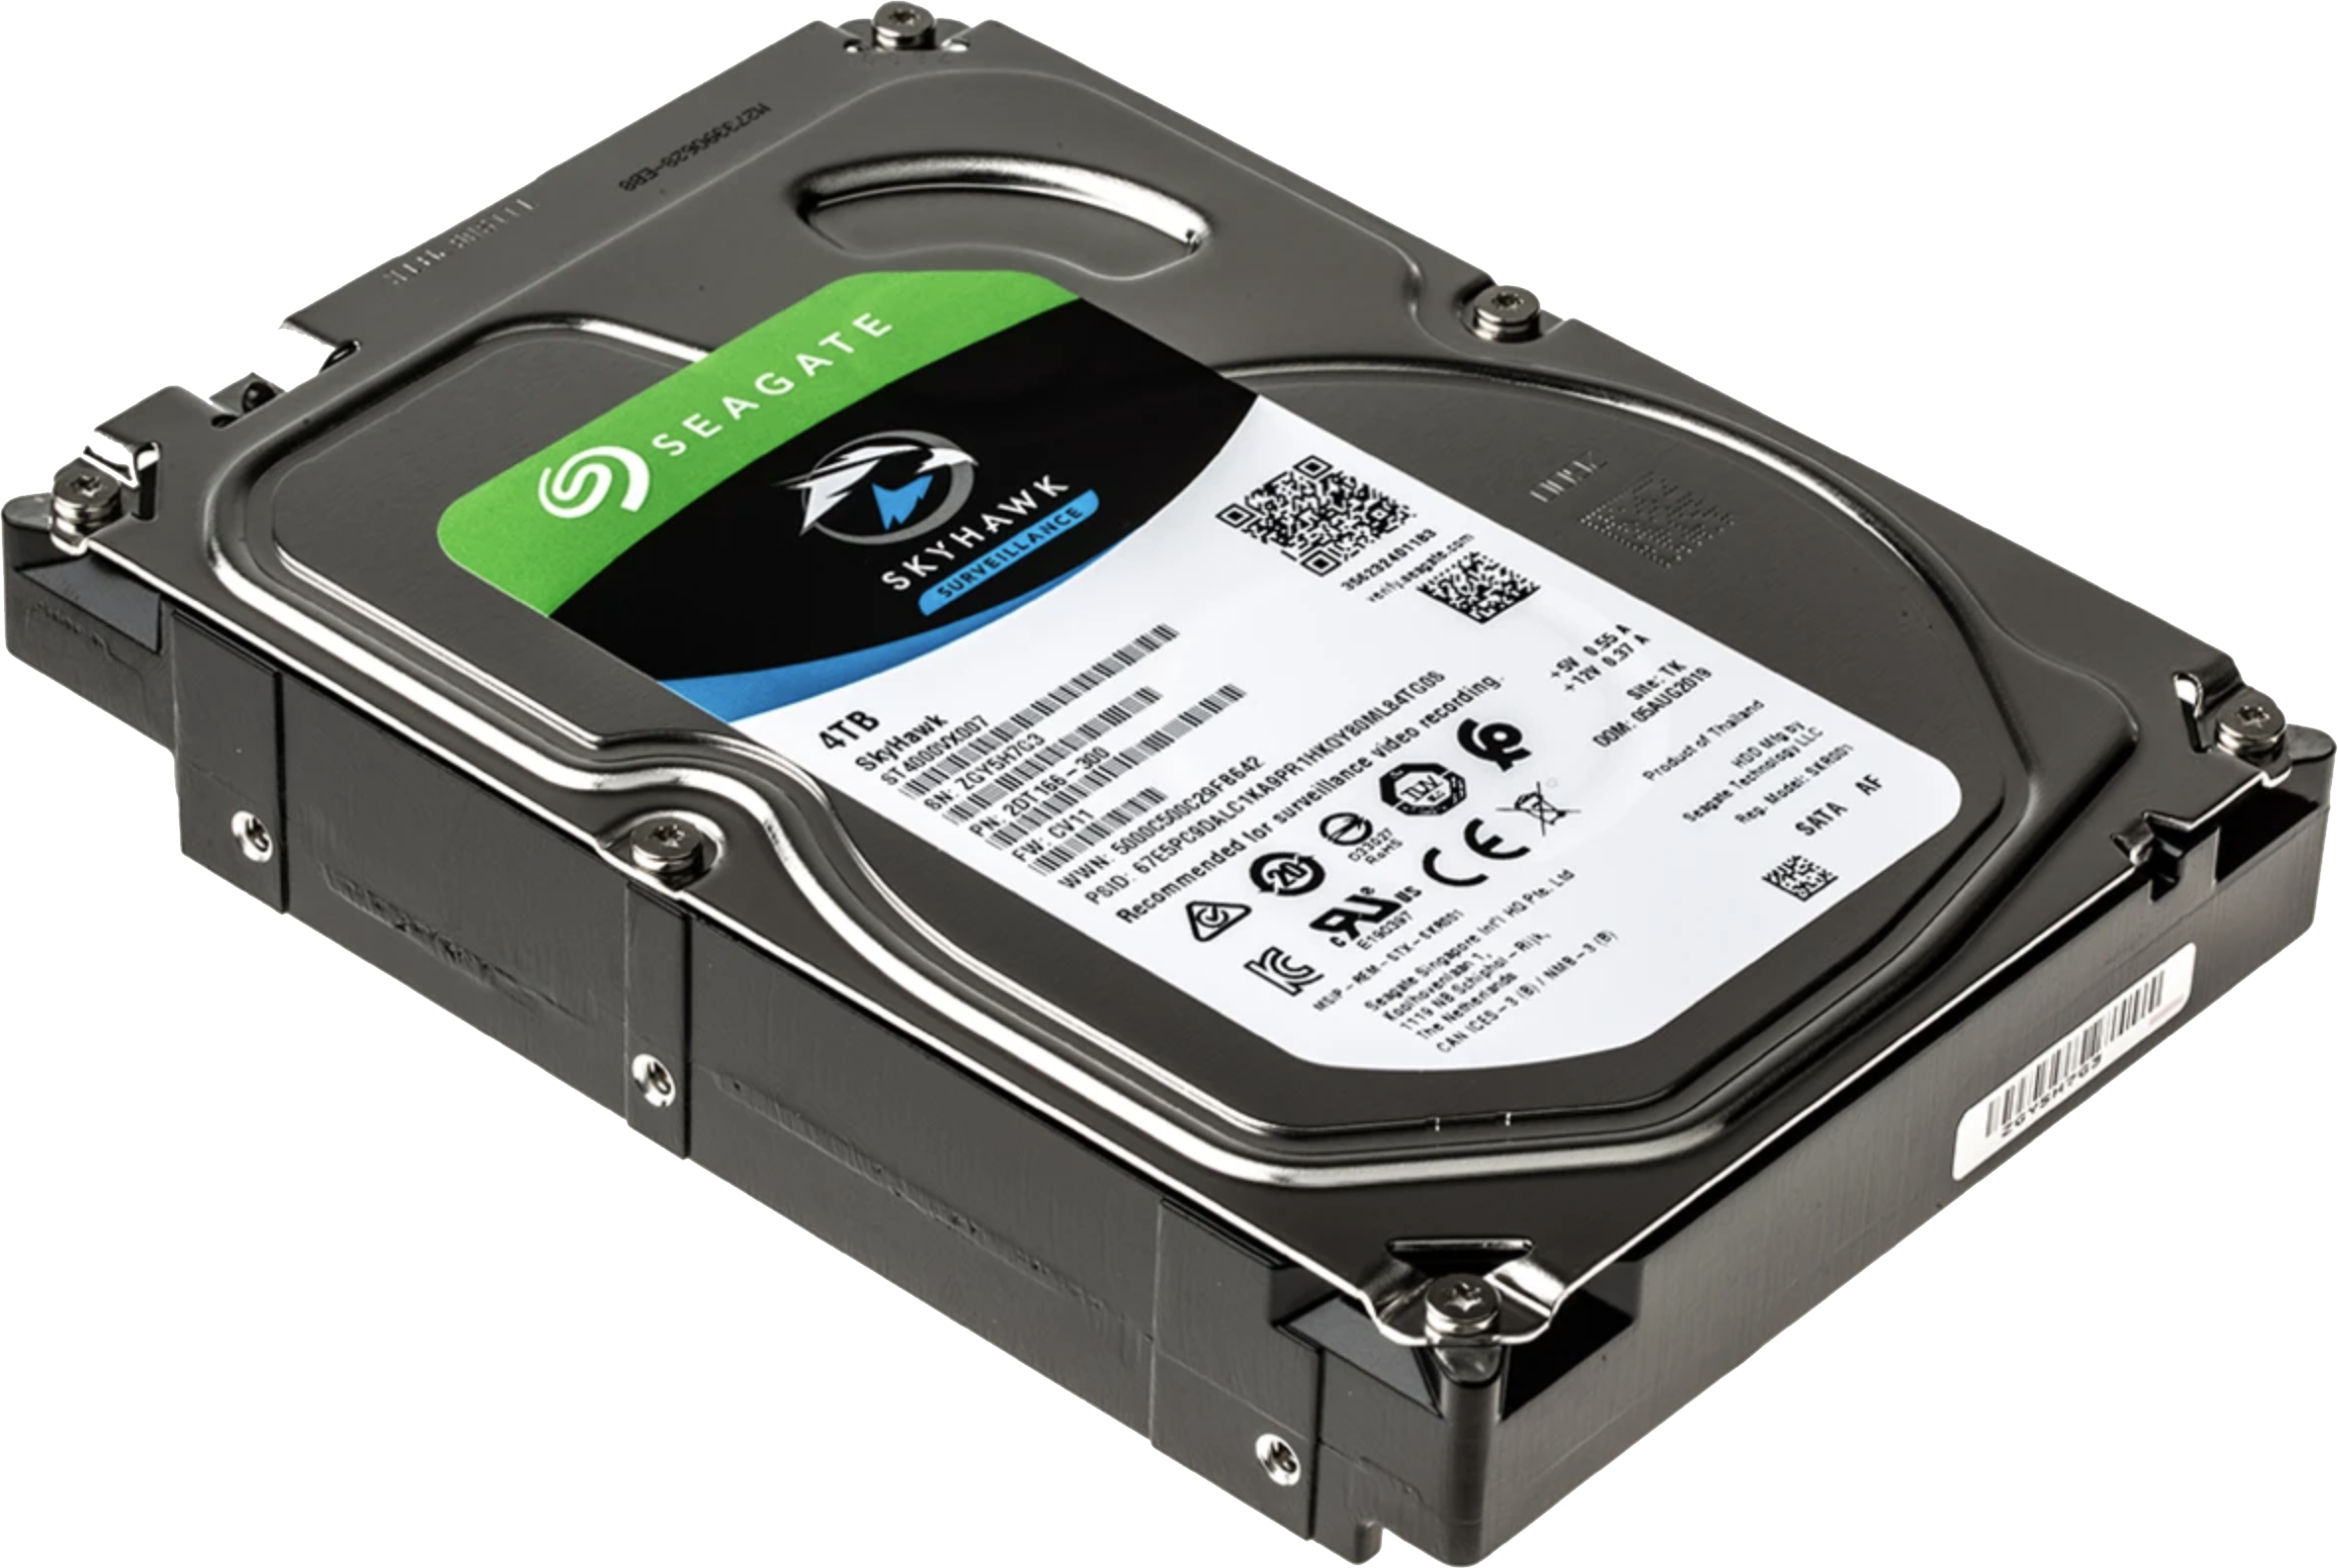
\includegraphics[width=0.6\linewidth]{Figures/harddrive.png}
        \end{wrapfigure}
           Still, although it might not feel so modern, sometimes \alert{if the data
           amount is large} and the \alert{network connections is bad} it might just be
           easiest to transfer the data physically by \alert{shipping a hard drive}.
        \end{block}
    \end{frame}
    \subsection{Commercial solutions}
    \begin{frame}
        \frametitle{Transferring data}
        \framesubtitle{Commercial solution}
        \begin{center}
            Sometimes there might be a commercial solution available
        \end{center}
        \uncover<2->{
        \begin{block}{IBM Aspera}
        \begin{wrapfigure}[4]{r}{0.4\textwidth}
        \vspace{-1.4\baselineskip}
        
\includegraphics[width=0.6\linewidth]{Figures/aspera-logo.png}
        \end{wrapfigure}
            IBM Aspera is a commercial solution for transferring large amount of data.
        \end{block}
        }
    \end{frame}

\section{Compression}
    \subsection{zip}

    \begin{frame}
        \frametitle{Compression}
        \framesubtitle{zip}
        \begin{block}{zip}
        \begin{wrapfigure}[4]{r}{0.2\textwidth}
        \centering
        \vspace{-6pt}
        
\includegraphics[width=0.55\linewidth]{Figures/zip.png}
        \end{wrapfigure}
            \mbox{}
            \begin{itemize}
                \item Appeared around \alert{1989}
                \item An archive format that \alert{can contain both files and directories} that \alert{can be compressed}
            \end{itemize}
            \mbox{}\vspace{-17pt}
            \begin{itemize}
                \item Built-in zip support in both Windows, Mac OS X and most free operating systems
                \item the name means ``move at high speed''
                \item an index allows for \alert{random access} of files from a zip archive
            \end{itemize}

        \end{block}
    \end{frame}

    \subsection{gz and tar.gz}
    \begin{frame}
        \frametitle{Compression}
        \framesubtitle{gz and tar.gz}
        \begin{block}{gzip (gz)}
        \begin{wrapfigure}[4]{r}{0.3\textwidth}
        \centering
        \vspace{-6pt}
        
\includegraphics[width=0.8\linewidth]{Figures/gzip.png}
        \end{wrapfigure}
            \mbox{}

        \begin{itemize}
            \item gzip is a way to compress files
            \item decompression can be done in a streaming fashion
        \end{itemize}
        \end{block}
    \end{frame}

    \begin{frame}
        \frametitle{Compression}
        \framesubtitle{gz and tar.gz}
        \begin{block}{z commands}
            There is a family of special commands to work with gzipped files:
            
            \begin{center}
            \begin{tabular}{rl}
                \texttt{zcat} & View a gzipped file \\
                \texttt{zless} & Browse a gzipped file \\
                \texttt{zgrep} & Search inside a gzipped file \\
                \texttt{zdiff} & Compare gzipped files \\
            \end{tabular}
            \end{center}
        \end{block}
    \end{frame}

\section{Storage}
    
    \subsection{Databases}
    \begin{frame}
        \frametitle{Databases}
        \framesubtitle{}

        \begin{block}{Databases}
        \small
            You are probably already familiar with \alert{relational databases} (\textit{e.g.}, MySQL) \\[10pt]

            But, with big data \alert{relational databases is not always going to cope}.\\[10pt]


            Although some can spread out over mulitple nodes, \textit{e.g.},
            Postgresql, there are other databases that might be more suited for
            big data, \textit{i.e.}, the \alert{noSQL databases}.
        \end{block}
    \end{frame}
    
    \begin{frame}
        \frametitle{Databases}
        \framesubtitle{NoSQL databases}

        There are databases that don't use SQL and relations. It is good to at
        least have heard about a few of them. Here are a few categories:

        \begin{block}{NoSQL Databases categories}
        \small
        \begin{itemize}
        \item \textbf{Document-oriented}: Stores data as entire documents (\textit{e.g.}, XML, JSON, YAML \ldots)
        \item \textbf{Key-value}: Stores data in associative arrays; what is sometimes
                         called \textit{dictionaries} or \textit{hashes}
        \item \textbf{Graph}: stores graph structures with \textit{nodes} and \textit{edges}
        \end{itemize}
        \end{block}
        There are many more\ldots
    \end{frame}
    
    \begin{frame}
        \frametitle{Databases}
        \framesubtitle{NoSQL databases}
        \begin{block}{Not as complex as relational databases}
            Since the \alert{NoSQL databases} are not as complex as relational
            databases they \alert{can sometimes handle big data much better}, for
            example the document database MongoDB was built to handle really
            large amounts of data.
        \end{block}
    \end{frame}

    \subsection{Local storage / Fast storage}
    \begin{frame}
        \frametitle{Storage when computing}
        \framesubtitle{Local storage / Fast storage}
        \begin{block}{Local storage}
        When working with big data it is important to think about where you
        data is situated. On big computer nodes you can have many different
        kind of storage. Maybe you have large slow storage located far away
        from the compute cores and smaller fast local scratch disks on the
        compute nodes. Depending on the algorithm it \alert{might be well worth
        copying the data to local scratch disks} first.
        \end{block}
    \end{frame}

\setbeamertemplate{background}{%
    \parbox[c][\paperheight]{\paperwidth}{%
        \vskip -8 ex \hskip -2 em
        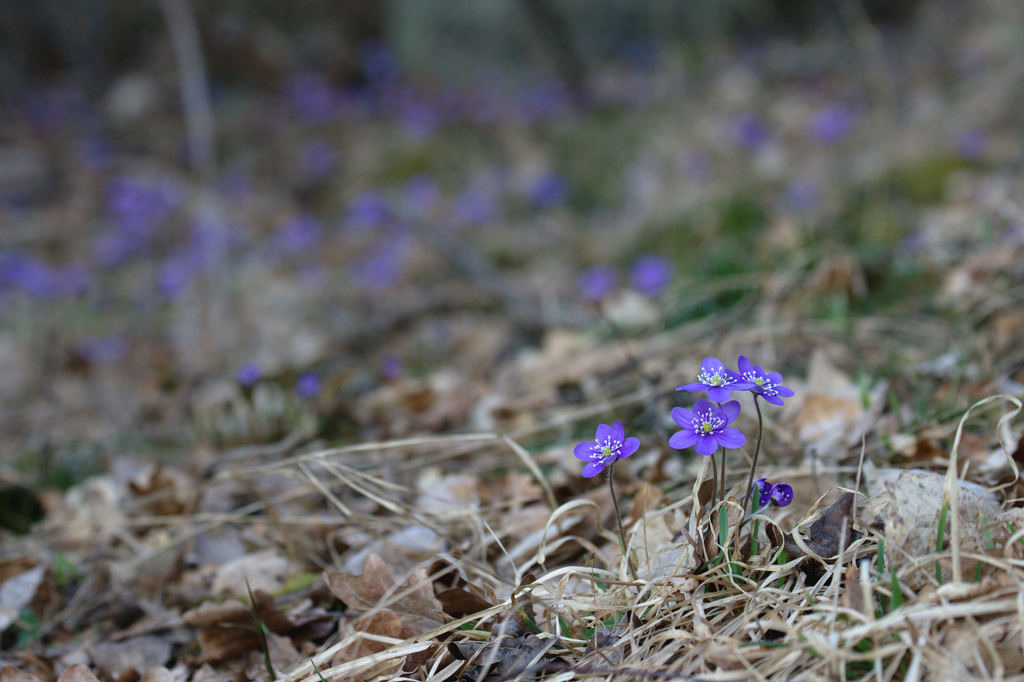
\includegraphics[height=1.5\paperheight]{Figures/blasippa.jpg}
    }   
    \parbox[c][\paperheight]{\paperwidth}{%
        \vskip 25 ex \hskip -40 em
        \color{white}\fbox{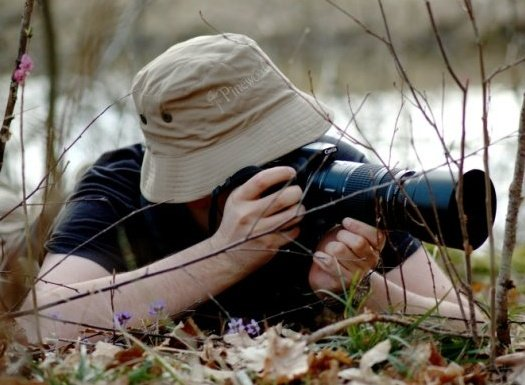
\includegraphics[height=0.37\paperheight]{Figures/me.jpg}}
    }   
}
\begin{frame}[plain]
    \vfill\hfill{\Huge\qquad\color{white} \zB Thank \zC you}\hfill\hfill\hfill\vfill
\end{frame}
\setbeamertemplate{background}{}
\end{document}
